\documentclass[11pt,a4paper]{article}

\usepackage[margin=22mm]{geometry}
\usepackage[T1]{fontenc}
\usepackage{lmodern}
\usepackage{xcolor}
\usepackage{microtype}
\usepackage{booktabs}
\usepackage{tabularx}
\usepackage{longtable}
\usepackage{array}
\usepackage{enumitem}
\usepackage{needspace}
\usepackage{listings}
\usepackage{fancyhdr}
\usepackage{titlesec}
\usepackage{graphicx}
\usepackage{tikz}
\usetikzlibrary{shapes.geometric, arrows.meta, positioning, fit, backgrounds, calc}
\usepackage{hyperref}

\definecolor{oaiblue}{HTML}{176B87}
\definecolor{oailight}{HTML}{EDF6F8}
\definecolor{oaiwarn}{HTML}{FFF4D6}
\definecolor{oaigreen}{HTML}{EAF6EE}
\definecolor{codebg}{HTML}{F5F5F5}
\definecolor{codeframe}{HTML}{C8C8C8}
\definecolor{oaipurple}{HTML}{8E44AD}
\definecolor{oaiorange}{HTML}{E67E22}
\definecolor{oaiteal}{HTML}{16A085}

\tikzset{
  container/.style={draw=oaiblue!60, fill=oailight!50, dashed, thick, rounded corners=6pt, inner sep=8pt},
  ducontainer/.style={draw=gray!60, fill=gray!5, dashed, thick, rounded corners=6pt, inner sep=8pt},
  corenode/.style={draw=oaiblue!90!black, fill=oaiblue, thick, rounded corners=4pt, minimum height=1cm, minimum width=2.2cm, align=center, font=\small, text=white},
  cunode/.style={draw=oaiblue!80!black, fill=oaiblue!75!black, thick, rounded corners=4pt, minimum height=1cm, minimum width=2.2cm, align=center, font=\small, text=white},
  dunode/.style={draw=oaipurple!90!black, fill=oaipurple, thick, rounded corners=4pt, minimum height=1cm, minimum width=2.2cm, align=center, font=\small, text=white},
  radionode/.style={draw=oaiorange!90!black, fill=orange!12, thick, rounded corners=4pt, minimum height=1cm, minimum width=2.2cm, align=center, font=\small},
  uenode/.style={draw=green!50!black, fill=oaigreen, thick, rounded corners=4pt, minimum height=1cm, minimum width=2.2cm, align=center, font=\small},
  modemnode/.style={draw=oaiteal!90!black, fill=oaiteal!12, thick, rounded corners=4pt, minimum height=1cm, minimum width=2.4cm, align=center, font=\small},
  busline/.style={-{Stealth[scale=1.1]}, thick, draw=oaiblue},
  f1line/.style={<->, {Stealth[scale=1.1]}-{Stealth[scale=1.1]}, very thick, draw=oaiblue},
  wgline/.style={<->, {Stealth[scale=1.1]}-{Stealth[scale=1.1]}, thick, dashed, draw=oaipurple},
  rfline/.style={<->, {Stealth[scale=1.1]}-{Stealth[scale=1.1]}, thick, dash pattern=on 4pt off 2.5pt, draw=oaiorange},
  hostlabel/.style={font=\scriptsize\bfseries, inner sep=1.5pt, fill=white, align=center},
  linklabel/.style={font=\scriptsize\bfseries, inner sep=1.5pt, fill=white, rounded corners=2pt, align=center},
  linknote/.style={font=\tiny, inner sep=1pt, fill=white, rounded corners=2pt, align=center}
}

\hypersetup{
  colorlinks=true,
  linkcolor=oaiblue,
  urlcolor=oaiblue,
  pdftitle={OAI CU/DU Lab Deployment and Operation Guide},
  pdfauthor={OAI CU/DU Lab}
}

\pagestyle{fancy}
\fancyhf{}
\fancyhead[L]{\small OAI CU/DU Lab}
\fancyhead[R]{\small Deployment and operation guide}
\fancyfoot[C]{\thepage}
\setlength{\headheight}{14pt}

\titleformat{\section}{\Large\bfseries\color{oaiblue}}{\thesection}{0.65em}{}
\titleformat{\subsection}{\large\bfseries}{\thesubsection}{0.6em}{}
\setlist{nosep,leftmargin=*}
\renewcommand{\arraystretch}{1.18}
\setlength{\parindent}{0pt}
\setlength{\parskip}{5pt}
\setcounter{tocdepth}{1}
\newcolumntype{L}[1]{>{\raggedright\arraybackslash}p{#1}}
\newcolumntype{C}[1]{>{\centering\arraybackslash}p{#1}}

\lstdefinestyle{lab}{
  basicstyle=\ttfamily\small,
  backgroundcolor=\color{codebg},
  frame=single,
  rulecolor=\color{codeframe},
  breaklines=true,
  columns=fullflexible,
  keepspaces=true,
  showstringspaces=false,
  aboveskip=7pt,
  belowskip=7pt
}
\lstset{style=lab}

\newcommand{\goodbox}[1]{%
  \par\medskip\noindent
  \fcolorbox{oaiblue}{oaigreen}{\parbox{0.94\linewidth}{\textbf{Validated result.} #1}}
  \par\medskip}
\newcommand{\notebox}[1]{%
  \par\medskip\noindent
  \fcolorbox{oaiblue}{oailight}{\parbox{0.94\linewidth}{\textbf{Operator note.} #1}}
  \par\medskip}
\newcommand{\warnbox}[1]{%
  \par\medskip\noindent
  \fcolorbox{orange!70!black}{oaiwarn}{\parbox{0.94\linewidth}{\textbf{Warning.} #1}}
  \par\medskip}

\begin{document}

\begin{titlepage}
  \centering
  \vspace*{25mm}
  {\Huge\bfseries\color{oaiblue} OAI CU/DU Lab\par}
  \vspace{5mm}
  {\LARGE Deployment and Operation Guide\par}
  \vspace{12mm}
  {\large A tutorial for reproducing the validated configurations\par}
  \vfill
  \begin{minipage}{0.82\textwidth}
    \notebox{This manual describes how to assemble and operate configurations that have worked in the lab. The two USRP B210 radios and the Quectel modem are shared resources. Moving them between hosts is a normal preparation step, not a failed validation.}
  \end{minipage}
  \vfill
  {\large Version: 29 July 2026\par}
  \vspace{4mm}
  {\small Canonical repository: \url{https://github.com/promaaa/oai-cu-du-lab/}\par}
  {\small GitHub wiki: \url{https://promaaa.github.io/oai-cu-du-lab/}\par}
\end{titlepage}

\tableofcontents
\clearpage

\section{Purpose and correct interpretation}

This document is an operating tutorial and technical reference reconciled with
repository commit
\texttt{b4652e386d40d9a3c9e1824a325faae5417d6f1d}. It is not a chronological
account of unfinished work. The public evidence record and maintained operator
matrix document successful demonstrations of the following
capabilities:

\begin{itemize}
  \item monolithic OAI 5G SA with a commercial phone;
  \item OAI CU/DU split over Ethernet;
  \item SIB8/PWS transported through F1 and observed on the Nothing Phone;
  \item F1-C and F1-U over a Wi-Fi GRE tunnel;
  \item F1 over a Quectel 5G packet session and WireGuard;
  \item access DU operation on MiniPC, Raspberry Pi 5, and Jetson Orin Nano;
  \item phone registration, PDU session, public internet, and throughput tests;
  \item OAI nrUE internet access over an NR radio link;
  \item repeatable launch, preflight, packet-placement, and rollback through the operator console.
\end{itemize}

\notebox{A recorded working capability is not fresh-run evidence. Every new
run must record the machine-side and phone-side gates separately. The current
baseline classifications in this guide therefore remain authoritative even
when the supported-capability matrix says \texttt{WORKING}.}

Only two combined-radio explorations did not reach the intended end-to-end
result:

\begin{enumerate}
  \item using one X310 for the fronthaul and backhaul functions together;
  \item using one B210 for the fronthaul and backhaul functions together.
\end{enumerate}

The X310 fronthaul and backhaul functions were usable separately. The combined
X310 topology failed. Likewise, a B210 works as an access radio and a B210 can
be used in a radio-link experiment, but one B210 could not simultaneously own
both independent OAI roles.

\section{Hardware pool and movement plan}

The lab has two USRP B210 radios and one Quectel modem. Before following a
tutorial, place the shared devices according to the selected scenario.

\begin{table}[ht]
\centering
\begin{tabularx}{\textwidth}{@{}L{29mm}X X@{}}
\toprule
Scenario & B210 placement & Quectel placement \\
\midrule
Monolithic reference & One B210 on the monolithic gNB host & Not required \\
Ethernet split & One B210 on the selected access-DU host & Not required \\
Wi-Fi GRE split & One B210 on the selected access-DU host & Not required \\
Quectel split & One B210 for the donor cell and one B210 for the access cell & On the access-DU side as the IP backhaul modem \\
Pi or Jetson DU & Move an available B210 to that host & Move only when testing Quectel backhaul \\
\bottomrule
\end{tabularx}
\end{table}

The configuration is designed to work correctly with either B210, including on
the Raspberry Pi and the Jetson, without relying on a specific device serial.
The operator console discovers the connected radio and generates the runtime
configuration. Discover the devices live before launch; do not rely on an old
USB topology.

\subsection{Physical move checklist}

\begin{enumerate}
  \item Stop the current scenario through the operator console.
  \item Confirm that no \texttt{nr-softmodem} process still owns the radio.
  \item Disconnect the B210 or Quectel only after the owning process is stopped.
  \item Connect the device to the target host.
  \item Confirm the B210 appears at USB SuperSpeed after UHD firmware load.
  \item Run UHD discovery and probe before starting OAI.
  \item Confirm the intended host, route, and interface with the console read-only checks.
\end{enumerate}

\begin{lstlisting}
uhd_find_devices
uhd_usrp_probe --args serial=<USRP_SERIAL>
lsusb -t
\end{lstlisting}

\section{Architecture}

\subsection{Monolithic reference}

The 5GC and gNB run on Firecell. The gNB owns a local B210 and serves the
commercial phone directly. This is the simplest reference for core, RF,
registration, PDU, internet, throughput, and PWS.

\begin{figure}[htbp]
\centering
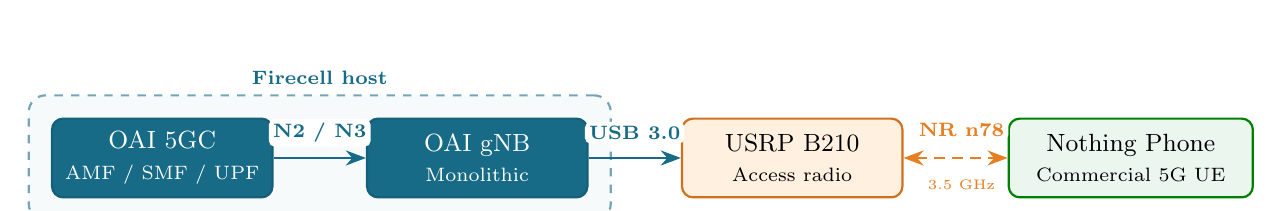
\begin{tikzpicture}
  \node[corenode, minimum width=28mm] at (0,0) (core)
    {OAI 5GC \\ \scriptsize AMF / SMF / UPF};
  \node[corenode, minimum width=28mm] at (4.0,0) (gnb)
    {OAI gNB \\ \scriptsize Monolithic};
  \node[radionode, minimum width=28mm] at (8.0,0) (b210)
    {USRP B210 \\ \scriptsize Access radio};
  \node[uenode, minimum width=31mm] at (12.3,0) (phone)
    {Nothing Phone \\ \scriptsize Commercial 5G UE};

  \begin{pgfonlayer}{background}
    \node[container, fit=(core) (gnb)] (firecell) {};
  \end{pgfonlayer}
  \node[hostlabel, text=oaiblue, anchor=south]
    at ([yshift=2pt]firecell.north) {Firecell host};

  \draw[busline] (core.east) -- (gnb.west);
  \node[linklabel, text=oaiblue] at (2.0,0.32) {N2 / N3};
  \draw[busline] (gnb.east) -- (b210.west);
  \node[linklabel, text=oaiblue] at (6.0,0.32) {USB 3.0};
  \draw[rfline] (b210.east) -- (phone.west);
  \node[linklabel, text=oaiorange] at (10.15,0.36) {NR n78};
  \node[linknote, text=oaiorange] at (10.15,-0.34) {3.5 GHz};
\end{tikzpicture}
\caption{Monolithic OAI 5G SA Reference Architecture}
\end{figure}

\subsection{CU/DU split}

Firecell hosts the OAI 5GC and CU. The selected DU host runs MAC, RLC, PHY, and
the access B210. F1-C uses SCTP. F1-U uses GTP-U over UDP.

\begin{figure}[htbp]
\centering
\resizebox{\linewidth}{!}{%
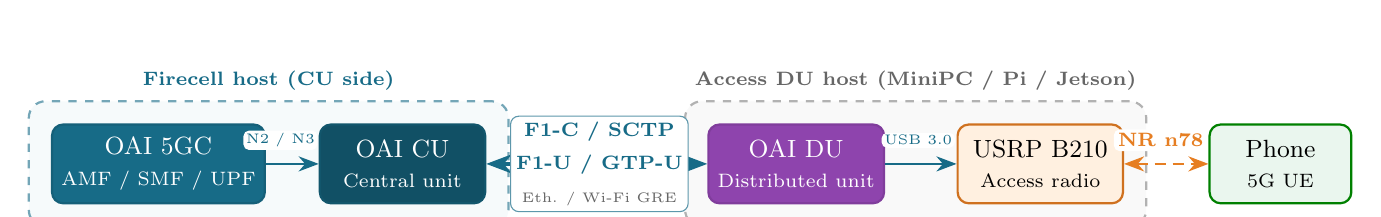
\begin{tikzpicture}
  \node[corenode, minimum width=21mm] at (0,0) (core)
    {OAI 5GC \\ \scriptsize AMF / SMF / UPF};
  \node[cunode, minimum width=21mm] at (3.1,0) (cu)
    {OAI CU \\ \scriptsize Central unit};
  \node[dunode, minimum width=21mm] at (8.1,0) (du)
    {OAI DU \\ \scriptsize Distributed unit};
  \node[radionode, minimum width=21mm] at (11.2,0) (b210)
    {USRP B210 \\ \scriptsize Access radio};
  \node[uenode, minimum width=18mm] at (14.25,0) (phone)
    {Phone \\ \scriptsize 5G UE};

  \begin{pgfonlayer}{background}
    \node[container, fit=(core) (cu)] (firecell) {};
    \node[ducontainer, fit=(du) (b210)] (duhost) {};
  \end{pgfonlayer}
  \node[hostlabel, text=oaiblue, anchor=south]
    at ([yshift=2pt]firecell.north) {Firecell host (CU side)};
  \node[hostlabel, text=gray!80!black, anchor=south]
    at ([yshift=2pt]duhost.north) {Access DU host (MiniPC / Pi / Jetson)};

  \draw[busline] (core.east) -- (cu.west);
  \node[linknote, text=oaiblue] at (1.55,0.30) {N2 / N3};

  \draw[f1line] (cu.east) -- (du.west);
  \node[
    draw=oaiblue!70,
    fill=white,
    rounded corners=3pt,
    minimum width=18mm,
    minimum height=11mm,
    align=center,
    inner sep=2pt,
    text=oaiblue
  ] at (5.60,0) {\scriptsize\bfseries F1-C / SCTP \\
                  \scriptsize\bfseries F1-U / GTP-U \\
                  \tiny\color{gray!80!black} Eth. / Wi-Fi GRE};

  \draw[busline] (du.east) -- (b210.west);
  \node[linknote, text=oaiblue] at (9.65,0.30) {USB 3.0};
  \draw[rfline] (b210.east) -- (phone.west);
  \node[linklabel, text=oaiorange] at (12.73,0.30) {NR n78};
\end{tikzpicture}%
}
\caption{OAI CU/DU Split Architecture}
\end{figure}

\subsection{Quectel wireless F1}

The Quectel path replaces the wired F1 transport with a 5G packet session and
a WireGuard overlay. The maintained workflow uses a monolithic donor gNB on
Firecell only to serve the Quectel modem. This donor has no F1 association.
The selected MiniPC, Raspberry Pi, or Jetson access DU is the only DU in this
workflow and serves the phone through the second B210.

\begin{figure}[htbp]
\centering
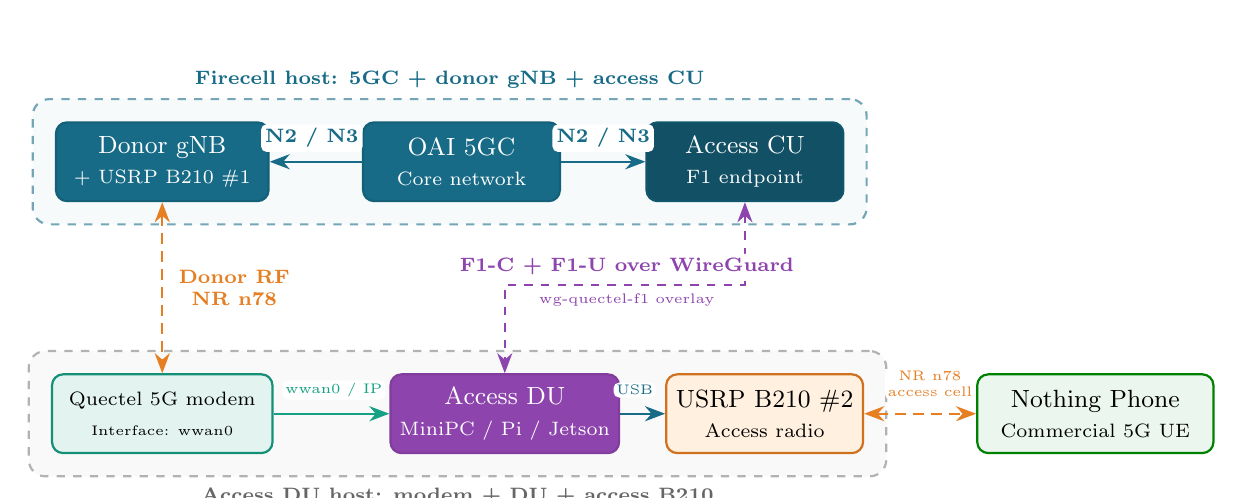
\begin{tikzpicture}
  % Firecell: donor service and access CU are separate OAI roles.
  \node[corenode, minimum width=27mm] at (0,2.7) (donor)
    {Donor gNB \\ \scriptsize + USRP B210 \#1};
  \node[corenode, minimum width=25mm] at (3.8,2.7) (core)
    {OAI 5GC \\ \scriptsize Core network};
  \node[cunode, minimum width=25mm] at (7.4,2.7) (cu)
    {Access CU \\ \scriptsize F1 endpoint};

  % Access host: modem provides the IP underlay; the DU owns the access radio.
  \node[modemnode, minimum width=28mm] at (0,-0.5) (modem)
    {\scriptsize Quectel 5G modem \\ \tiny Interface: wwan0};
  \node[dunode, minimum width=25mm] at (4.35,-0.5) (du)
    {Access DU \\ \scriptsize MiniPC / Pi / Jetson};
  \node[radionode, minimum width=25mm] at (7.65,-0.5) (b210)
    {USRP B210 \#2 \\ \scriptsize Access radio};
  \node[uenode, minimum width=30mm] at (11.85,-0.5) (phone)
    {Nothing Phone \\ \scriptsize Commercial 5G UE};

  \begin{pgfonlayer}{background}
    \node[container, fit=(donor) (core) (cu)] (firecell) {};
    \node[ducontainer, fit=(modem) (du) (b210)] (duhost) {};
  \end{pgfonlayer}
  \node[hostlabel, text=oaiblue, anchor=south]
    at ([yshift=2pt]firecell.north)
    {Firecell host: 5GC + donor gNB + access CU};
  \node[hostlabel, text=gray!80!black, anchor=north]
    at ([yshift=-2pt]duhost.south)
    {Access DU host: modem + DU + access B210};

  \draw[busline] (core.west) -- (donor.east);
  \node[linklabel, text=oaiblue] at (1.9,3.0) {N2 / N3};
  \draw[busline] (core.east) -- (cu.west);
  \node[linklabel, text=oaiblue] at (5.6,3.0) {N2 / N3};

  \draw[rfline] (donor.south) -- (modem.north);
  \node[linklabel, text=oaiorange, anchor=west] at (0.15,1.1)
    {Donor RF \\ NR n78};

  \draw[wgline] (cu.south) -- ++(0,-1.05) -| (du.north);
  \node[linklabel, text=oaipurple] at (5.9,1.37)
    {F1-C + F1-U over WireGuard};
  \node[linknote, text=oaipurple] at (5.9,0.94)
    {wg-quectel-f1 overlay};

  \draw[-{Stealth[scale=1.1]}, thick, draw=oaiteal]
    (modem.east) -- (du.west);
  \node[linknote, text=oaiteal] at (2.18,-0.20) {wwan0 / IP};
  \draw[busline] (du.east) -- (b210.west);
  \node[linknote, text=oaiblue] at (6.0,-0.20) {USB};
  \draw[rfline] (b210.east) -- (phone.west);
  \node[linknote, text=oaiorange] at (9.75,-0.12)
    {NR n78 \\ access cell};
\end{tikzpicture}
\caption{Quectel 5G Wireless Backhaul \& WireGuard F1 Architecture}
\end{figure}

\warnbox{The deprecated donor-DU-over-local-F1 experiment is not the
maintained Quectel workflow. The modem must not use the access cell as its own
backhaul; that creates an unsupported circular dependency.}

\section{Supported capabilities and current baselines}

The maintained operator console exposes Ethernet, Wi-Fi GRE, and Quectel with
WireGuard for MiniPC, Raspberry Pi, and Jetson access DUs. These nine
combinations, the monolithic reference, SIB8 and PWS, phone service, clean
stop, and Ethernet rollback are recorded as working capabilities.

\begin{table}[ht]
\centering
\begin{tabularx}{\textwidth}{@{}X C{26mm} C{26mm} C{38mm}@{}}
\toprule
Access DU & Ethernet & Wi-Fi GRE & Quectel/WireGuard \\
\midrule
MiniPC & \texttt{WORKING} & \texttt{WORKING} & \texttt{WORKING} \\
Raspberry Pi & \texttt{WORKING} & \texttt{WORKING} & \texttt{WORKING} \\
Jetson & \texttt{WORKING} & \texttt{WORKING} & \texttt{WORKING} \\
\bottomrule
\end{tabularx}
\end{table}

The table below is the stricter current evidence view. Historical throughput
is context, not a ceiling or a substitute for a controlled rerun.

\begin{longtable}{@{}L{35mm}L{29mm}L{34mm}L{54mm}@{}}
\toprule
Scenario & Role & Recorded result & Current classification \\
\midrule
\endfirsthead
\toprule
Scenario & Role & Recorded result & Current classification \\
\midrule
\endhead
Monolithic OAI & Reference only & About 150 Mbps historically &
\texttt{PARTIAL}: machine-side reference reproduced 14 July 2026; phone gates not rerun \\
MiniPC Ethernet CU/DU + SIB8 & Canonical rollback & About 19--23 Mbps historically &
\texttt{BLOCKED}: B210 was not on MiniPC during the latest rollback attempt \\
Wi-Fi GRE CU/DU + SIB8 & Wireless candidate & About 12 Mbps historically &
\texttt{HISTORICAL}: requires fresh validation \\
Raspberry Pi Ethernet CU/DU & Lightweight candidate & About 18--23 Mbps historically &
\texttt{HISTORICAL}: requires fresh validation \\
Jetson Ethernet CU/DU & Embedded candidate & 6.5--7.3 Mbps in an earlier run &
\texttt{PARTIAL}: current phone and rollback gates remain incomplete \\
Quectel/WireGuard F1 & Target wireless backhaul & No accepted end-to-end result &
\texttt{BLOCKED}: the maintained donor/access topology requires fresh proof \\
\bottomrule
\end{longtable}

\warnbox{Do not promote a historical throughput number to a current PASS.
A full PASS requires all ten validation gates in Section~\ref{sec:validation}
from the same controlled run.}

\section{Prepare the repository and hosts}

\subsection{Local configuration}

The operator workstation requires Node.js 18 or newer, OpenSSH, lab network
access, SSH keys, and a private environment file. Clone the repository and
create that ignored local file with private permissions.

\begin{lstlisting}
git clone https://github.com/promaaa/oai-cu-du-lab.git
cd oai-cu-du-lab
mkdir -p conf/local
cp conf/lab.env.example conf/local/lab.env
chmod 600 conf/local/lab.env
\end{lstlisting}

Edit \texttt{conf/local/lab.env} for the current host addresses and runtime
paths. Use SSH keys or an agent. Never store passwords, UE authentication
values, WireGuard private keys, or subscriber dumps in Git.

The file may instead remain outside the repository:

\begin{lstlisting}
./oai-lab --env="$HOME/private/lab.env" --check-local-setup
\end{lstlisting}

The maintained split baseline uses external OAI source pinned at:

\begin{lstlisting}
102965a669b9444857c27843ec8ce62780bf9d37
\end{lstlisting}

Record the repository commit, actual CU and DU OAI commits, and local patch
state before a run. Required OAI modifications must be applied from
feature-separated patches under \texttt{patches/}. Generated runtime
configuration remains outside Git.

\subsection{Read-only checks}

\begin{lstlisting}
./oai-lab --help
./oai-lab --check-local-setup
node scripts/tests/oai-lab-static.test.mjs

./oai-lab --minipc-ethernet --verify
./oai-lab --status
./oai-lab --logs
\end{lstlisting}

\texttt{--check-local-setup} and the static suite do not contact the lab.
\texttt{--verify}, \texttt{--status}, and \texttt{--logs} contact the
configured hosts. Static tests prove CLI and menu dispatch plus
external-command blocking; they are not radio or phone evidence.

\notebox{\texttt{./oai-lab} is the only supported operator entry point.
Files under \texttt{scripts/lib/} are internal implementation details and
must not be launched directly.}

\section{Run the monolithic reference}

Use this mode first when checking the core, RF, subscriber, PWS, or user plane.
It removes F1 transport from the diagnostic path.

\begin{lstlisting}
./oai-lab --start-mono
./oai-lab --logs
\end{lstlisting}

\begin{enumerate}
  \item Connect the Firecell B210, stop any split scenario, and start monolithic mode.
  \item Wait for core health, NG setup, RF readiness, and synchronization.
  \item Toggle airplane mode once; verify PWS, registration, PDU session, and internet.
  \item Record DL/UL throughput, then stop and check for process residue.
\end{enumerate}

The historical reference was about 150 Mbps. The current baseline is
\texttt{PARTIAL} until the phone gates are rerun.

\section{Run Ethernet CU/DU}

Place either available B210 on the selected DU host. The operator console discovers its
serial and injects it into the runtime configuration. Firecell runs the 5GC
and CU; Ethernet carries F1-C and F1-U.

\begin{lstlisting}
./oai-lab --minipc-ethernet --start-ethernet
./oai-lab --pi-ethernet --start-ethernet
./oai-lab --jetson-ethernet --start-ethernet
\end{lstlisting}

Run only the command for the chosen host, then verify:

\begin{enumerate}
  \item F1 setup, SCTP, and GTP-U use the selected Ethernet path.
  \item The B210 reaches RF-ready and synchronized state.
  \item The phone receives PWS, registers, obtains a PDU session, and reaches the internet.
  \item DL/UL throughput and clean stop are recorded.
\end{enumerate}

Historical DL context is about 19--23 Mbps on MiniPC, about 18--23 Mbps on Pi,
and 6.5--7.3 Mbps on Jetson. None of those numbers replaces a fresh result.
On Pi, check the performance governor and throttling. On Jetson, use the SCTP
kernel, maximum-performance mode, CPU affinity, and separated USB IRQs.

\section{Run Wi-Fi GRE F1}

This profile keeps the F1 endpoint addresses but carries F1 over the Wi-Fi
underlay and \texttt{test-gre} tunnel.

\begin{lstlisting}
./oai-lab --minipc-wifi-gre --start-wifi-gre
./oai-lab --pi-wifi-gre --start-wifi-gre
./oai-lab --jetson-wifi-gre --start-wifi-gre
\end{lstlisting}

Run only the selected host profile. Before launch, preserve management access
and confirm symmetric Wi-Fi/GRE routing. During the run, verify SCTP and GTP-U
on \texttt{test-gre}, absence of F1 on the direct Ethernet path, and the full
phone acceptance sequence from the validation protocol. The current evidence
classification is \texttt{HISTORICAL}; the roughly 12 Mbps record requires a
fresh controlled rerun.

\section{Run Quectel/WireGuard F1}

This profile requires two independent cells: the monolithic Firecell donor gNB
serves the Quectel modem, while the selected access DU and second B210 serve
the phone. F1 crosses \texttt{wg-quectel-f1} over the detected Quectel data
interface, normally \texttt{wwan0}; donor and access cell identities must
remain distinct.

\begin{lstlisting}
./oai-lab --minipc-quectel-wg --start-quectel-wg
./oai-lab --pi-quectel-wg --start-quectel-wg
./oai-lab --jetson-quectel-wg --start-quectel-wg
\end{lstlisting}

Run only the selected host profile, then verify:

\begin{enumerate}
  \item the donor cell is operational and the modem registers on it;
  \item \texttt{wwan0} has a packet session and WireGuard tunnel ping succeeds;
  \item F1-C/F1-U are inside WireGuard and encrypted outer traffic is on \texttt{wwan0};
  \item the phone passes PWS, registration, PDU, internet, and throughput gates.
\end{enumerate}

The current baseline records no accepted end-to-end result for this maintained
topology. Treat machine-side WireGuard or F1 success as partial evidence only;
do not claim a full PASS until the modem donor-cell identity, access-cell phone
traffic, PWS, registration, PDU, internet, throughput, clean stop, and Ethernet
rollback are all captured in one controlled run.

\section{Send and validate PWS/SIB8}

Use \texttt{./oai-lab}, select \texttt{Change PWS warning text for all TUI
configs}, and enter only sanitized warning content. Restart the selected
scenario because OAI reads the warning file at startup. The CU sends the
warning through F1AP, the DU schedules SIB8, and the phone displays the alert.

Acceptance is simple: confirm the phone is on the intended access cell and
visually observe the warning. CU/DU log messages alone are not a PASS.

\section{Performance tuning}

\subsection{BLER and MCS}

The operator console generates per-run configuration from the selected host,
transport, live B210 serial, and validated defaults. The current default radio
window and TCP clamp are:

\begin{lstlisting}
dl_bler_target_lower = 0.45
dl_bler_target_upper = 0.65
ul_bler_target_lower = 0.25
ul_bler_target_upper = 0.45
tcp_mss_clamp        = 1200
\end{lstlisting}

Ethernet launch first tests whether the full path can carry MTU 9000 before
raising both F1 interfaces. If that test fails, the console keeps jumbo frames
disabled and uses TCP MSS clamping. Non-Ethernet modes skip jumbo frames.

The default MCS range is asymmetric: DL 10--18 and UL 5--28 for MiniPC and Pi;
Jetson uses DL 10--28 and UL 5--28. The \texttt{--force-mcs} option raises the
minimums to DL 12 and UL 8. Use these maintained defaults first, then change
them only from fresh RF, BLER, HARQ, overflow, and throughput evidence.

\subsection{Jetson USB and CPU placement}

The Jetson requires a clean USB3 path. Keep the DU away from CPU 0 and place
the active xHCI interrupt on CPU 0. Select the interrupt that is actually
increasing, not simply the first USB-looking line in \texttt{/proc/interrupts}.

\begin{lstlisting}
DU process: CPUs 1-5
active xHCI IRQ: CPU 0
usbfs_memory_mb: 1000
power mode: MAXN_SUPER
\end{lstlisting}

\section{The two unsuccessful combined-radio explorations}

\subsection{X310 used for fronthaul and backhaul together}

The X310 was explored in both roles. The fronthaul function and backhaul
function could be run separately at a feasible configuration. The attempt to
combine both roles into one end-to-end fronthaul/backhaul system did not work.

The strongest measured transport limitation appeared at 106 PRB. The host to
X310 path negotiated only 1 GbE. Both the reduced 46.08 MSps mode and native
61.44 MSps mode overflowed after RF-ready. A new cable rated far above 1 Gb/s
did not change the negotiated end-to-end path, so it did not fix the problem.

\begin{table}[ht]
\centering
\caption{X310 exploration summary}
\begin{tabularx}{\textwidth}{@{}L{42mm}X@{}}
\toprule
Test & Result \\
\midrule
X310 fronthaul role alone & Functional at a feasible standalone profile \\
X310 backhaul role alone & Functional as a separate role \\
Combined fronthaul and backhaul & Failed to reach the intended end-to-end result \\
106 PRB over negotiated 1 GbE & UHD overflow and RFNoC timeout \\
Higher-rated cable & Did not raise the negotiated path or remove overflow \\
\bottomrule
\end{tabularx}
\end{table}

The next meaningful combined X310 attempt must first prove a real high-speed
NIC, switch, MTU, and UHD streaming path. Cable labeling alone is not proof.

\subsection{One B210 used for fronthaul and backhaul together}

The single-B210 experiment tried to use the two RF chains for independent
access and backhaul systems. Two independent OAI processes could not safely
open the same UHD device, and both chains shared device-level clock and local
oscillator constraints. A single-owner broker moved IQ blocks without queue
drops, but the complete donor PRACH, registration, active F1, and phone service
chain did not close.

This does not invalidate B210 access operation or B210 radio-link operation.
It shows that one B210 cannot be treated as two independent radios by two OAI
roles without deeper device-layer integration.

\section{Validation protocol}
\label{sec:validation}

For every tutorial, record these gates separately:

\begin{longtable}{@{}L{42mm}L{115mm}@{}}
\toprule
Gate & Required evidence \\
\midrule
\endfirsthead
\toprule
Gate & Required evidence \\
\midrule
\endhead
Host and process health & Correct hosts, commits, processes, core containers, and exclusive ownership \\
NG and F1-C & NG setup and SCTP association on the selected path \\
F1-U & GTP-U sockets and packets on the selected path \\
RF and timing & UHD device, RF ready, sync, and bounded overflow behavior \\
PWS & Warning visible on the commercial phone \\
Registration & UE visible as registered in the active core \\
PDU session & Live data UE address and session rules \\
External-DN & Ping to the live UE address with recorded loss and RTT \\
Phone internet & Web or application traffic through the 5G bearer \\
Throughput & Timestamped DL and UL result with units \\
Stop and rollback & No stale process, route, firewall, MTU, GRE, or WireGuard state \\
\bottomrule
\end{longtable}

Runtime evidence is stored outside the repository:

\begin{lstlisting}
~/.local/state/oai-cu-du-lab/runs/
\end{lstlisting}

Set \texttt{OAI\_LAB\_STATE\_DIR} to choose another private location. Commit
only sanitized conclusions.

\section{Recovery and troubleshooting}

\begin{longtable}{@{}L{47mm}L{110mm}@{}}
\toprule
Symptom & First action \\
\midrule
\endfirsthead
\toprule
Symptom & First action \\
\midrule
\endhead
PWS but no 5G service & Watch RACH and initial UL RRC while toggling airplane mode once \\
UE registered but no PDU & Inspect AMF, SMF, NRF, and DNN state before restarting only the failing service \\
PDU exists but no phone internet & Confirm live UE IP, external-DN ping, APN, NAT, and UPF route \\
B210 at 480M & Probe with UHD and verify runtime re-enumeration at 5000M \\
Jetson overflow or loss & Check active xHCI IRQ placement and the overflow delta during traffic \\
X310 106 PRB overflow & Stop and prove negotiated transport above 1 GbE first \\
F1 on the wrong interface & Stop through the operator console, inspect routes and tunnels, then relaunch \\
\bottomrule
\end{longtable}

Recovery order:

\begin{enumerate}
  \item Stop the selected scenario through the operator console.
  \item Confirm remaining softmodem and core processes.
  \item Remove only scenario-owned route, tunnel, firewall, and MTU changes.
  \item Preserve management connectivity.
  \item Move the shared hardware to the rollback arrangement.
  \item Restore the MiniPC Ethernet profile and validate it end to end.
\end{enumerate}

\section{Public evidence provenance}

This tutorial relies only on the sanitized evidence published in
\texttt{docs/evidence/}, the pinned artifact manifest, and the maintained
baseline and status documents. Private laboratory notes, raw captures,
operational addresses, and intermediate interpretations are intentionally
outside the publication corpus.

\section{Quick command reference}

\begin{lstlisting}
# Interactive operator interface
./oai-lab

# Read-only checks
./oai-lab --help
./oai-lab --check-local-setup
./oai-lab --status
./oai-lab --logs
./oai-lab --minipc-ethernet --verify

# MiniPC profiles
./oai-lab --minipc-ethernet --start-ethernet
./oai-lab --minipc-wifi-gre --start-wifi-gre
./oai-lab --minipc-quectel-wg --start-quectel-wg

# Raspberry Pi profiles
./oai-lab --pi-ethernet --start-ethernet
./oai-lab --pi-wifi-gre --start-wifi-gre
./oai-lab --pi-quectel-wg --start-quectel-wg

# Jetson profiles
./oai-lab --jetson-ethernet --start-ethernet
./oai-lab --jetson-wifi-gre --start-wifi-gre
./oai-lab --jetson-quectel-wg --start-quectel-wg

# Local static audit, no lab contact
node scripts/tests/oai-lab-static.test.mjs
\end{lstlisting}

\section{Conclusion}

The project records a functioning multi-configuration OAI platform.
Monolithic, Ethernet split, Wi-Fi GRE, Quectel/WireGuard, Pi DU, Jetson DU,
PWS, phone user plane, and software UE internet have all worked. The shared
hardware must be moved to assemble the selected configuration, which is normal
for this lab. These capability records do not replace the current baseline
classifications or the need for fresh evidence.

The two negative results are narrow and useful: one X310 did not complete the
combined fronthaul/backhaul topology even though the roles worked separately,
and one B210 did not complete simultaneous fronthaul and backhaul. These results
define hardware and transport boundaries; they do not redefine the successful
configurations as failures.

\end{document}
